%%%%%%%%%%%%%%%%%%%%%%%%%%%%%%%%%%%%%%%%%%%%%%%%%%%%%%%%%%%%%%%
%
% Welcome to writeLaTeX --- just edit your LaTeX on the left,
% and we'll compile it for you on the right. If you give
% someone the link to this page, they can edit at the same
% time. See the help menu above for more info. Enjoy!
%
%%%%%%%%%%%%%%%%%%%%%%%%%%%%%%%%%%%%%%%%%%%%%%%%%%%%%%%%%%%%%%%

% --------------------------------------------------------------
% This is all preamble stuff that you don't have to worry about.
% Head down to where it says "Start here"
% --------------------------------------------------------------
 
\documentclass[12pt]{article}
 
\usepackage[margin=1in]{geometry}
\usepackage{amsmath,amsthm,amssymb}

\usepackage{listings}
\usepackage{xcolor}
\usepackage{graphicx}
\graphicspath{{./images/}}

%New colors defined below
\definecolor{codegreen}{rgb}{0,0.6,0}
\definecolor{codegray}{rgb}{0.5,0.5,0.5}
\definecolor{codepurple}{rgb}{0.58,0,0.82}
\definecolor{backcolour}{rgb}{0.95,0.95,0.92}

%Code listing style named "mystyle"
\lstdefinestyle{mystyle}{
  backgroundcolor=\color{backcolour}, commentstyle=\color{codegreen},
  keywordstyle=\color{magenta},
  numberstyle=\tiny\color{codegray},
  stringstyle=\color{codepurple},
  basicstyle=\ttfamily\footnotesize,
  breakatwhitespace=false,         
  breaklines=true,                 
  captionpos=b,                    
  keepspaces=true,                 
  numbers=left,                    
  numbersep=5pt,                  
  showspaces=false,                
  showstringspaces=false,
  showtabs=false,                  
  tabsize=2
}

%"mystyle" code listing set
\lstset{style=mystyle}

 
\newcommand{\N}{\mathbb{N}}
\newcommand{\Z}{\mathbb{Z}}
 
\newenvironment{theorem}[2][Theorem]{\begin{trivlist}
\item[\hskip \labelsep {\bfseries #1}\hskip \labelsep {\bfseries #2.}]}{\end{trivlist}}
\newenvironment{lemma}[2][Lemma]{\begin{trivlist}
\item[\hskip \labelsep {\bfseries #1}\hskip \labelsep {\bfseries #2.}]}{\end{trivlist}}
\newenvironment{exercise}[2][Exercise]{\begin{trivlist}
\item[\hskip \labelsep {\bfseries #1}\hskip \labelsep {\bfseries #2.}]}{\end{trivlist}}
\newenvironment{problem}[2][Problem]{\begin{trivlist}
\item[\hskip \labelsep {\bfseries #1}\hskip \labelsep {\bfseries #2.}]}{\end{trivlist}}
\newenvironment{question}[2][Question]{\begin{trivlist}
\item[\hskip \labelsep {\bfseries #1}\hskip \labelsep {\bfseries #2.}]}{\end{trivlist}}
\newenvironment{corollary}[2][Corollary]{\begin{trivlist}
\item[\hskip \labelsep {\bfseries #1}\hskip \labelsep {\bfseries #2.}]}{\end{trivlist}}

\newenvironment{solution}{\begin{proof}[Solution]}{\end{proof}}
 
\begin{document}
 
% --------------------------------------------------------------
%                         Start here
% --------------------------------------------------------------
 
\title{Test 1}%replace X with the appropriate number
\author{Mengxiang Jiang\\ %replace with your name
CSEN 5322 Operating Systems} %if necessary, replace with your course title
 
\maketitle
 
\begin{problem}{1} %You can use theorem, exercise, problem, or question here.  Modify x.yz to be whatever number you are proving
    (a) What is multiprogramming? (b) What is the key difference between a trap
    and an interrupt?

    (a) Multiprogramming is the ability for a user to run multiple programs at once.

    (b) A trap is an instruction to switch the execution mode from user to kernel mode. An interrupt is a signal sent to the CPU usually when an I/O process has finished.

\end{problem}

\begin{problem}{2} %You can use theorem, exercise, problem, or question here.  Modify x.yz to be whatever number you are proving
    In Figure below, three process states and four transitions are shown. What are the
    circumstances in which either or both of the missing transitions might occur?
    \begin{figure}[ht]
        \centering
        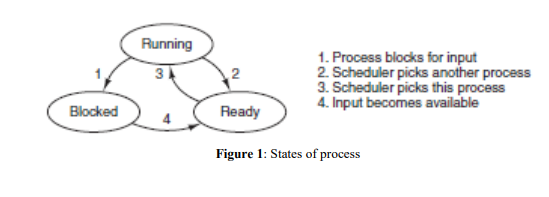
\includegraphics[width=\textwidth]{problem2}
    \end{figure}

    One missing transition is from Blocked to Running. This cannot happen since Blocked means it is currently unable to run until some external event happens, and when that something happens, it will go to Ready rather than Running. 
    Of course, if there are no processes/threads in the Ready state, it will get immediately picked up and go to Running state, as if it transitioned to Running directly, but it still must go to Ready state first.

    The second missing transition is from Ready to Blocked. This cannot happen since Ready means it is runnable but not currently running, so it cannot possibly be determined to be blocked on some external event. Of course, if it is picked up by Running and immediately requires I/O or some process that will block it, it will seem like it transitioned from Ready to Blocked, even though in actuality it first transitioned to Running first.
\end{problem}
 
\begin{problem}{3}
    In Figure below, a multithreaded Web server is shown. If the only way to read from a file is
    the normal blocking read system call, do you think user-level threads or kernel-level threads are being used
    for the Web server? Why?
    \begin{figure}[ht]
        \centering
        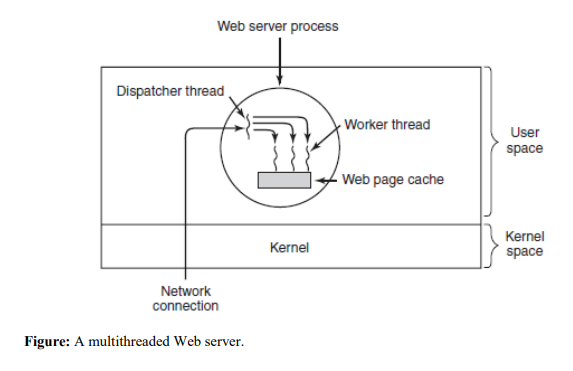
\includegraphics[width=\textwidth]{problem3}
    \end{figure}

    Both user-level and kernel-level threads are used, since the user-level threads can read the local cache of a file if it exists, and if its not in the cache, then a kernel level thread will be used to fetch the file from disk.
\end{problem}

\begin{problem}{4}
    (a) The aging algorithm with a= 1/2 is being used to predict run times. The previous
four runs, from oldest to most recent, are 80, 40, 80, and 30 msec. What are the predictions of the next
time? (you must show your calculations)\\\\
Prediction 1 is just 80.\\
Prediction 2 is $\frac{1}{2}*(80) + \frac{1}{2}*40 = 60$\\
Prediction 3 is $\frac{1}{2}*(60) + \frac{1}{2}*80 = 70$\\
Prediction 4 is $\frac{1}{2}*(70) + \frac{1}{2}*30 = 50$\\
Therefore the sequence of predictions is 80, 60, 70, 50, so 50 is the next prediction.\\\\
(b) If a system has only two processes, does it make sense to use a barrier to synchronize them? Why or
why not?\\\\
Yes, if you need to synchronize the two processes when one is faster than the other, a barrier is the ideal solution since it allows blocking without busy waiting (wasting cpu). Although strict alternation can also work and is simpler to implement, it will waste cpu by busy waiting.
\end{problem}


\begin{problem}{5}
    Suppose that we have a message-passing system using mailboxes. When sending to a full
    mailbox or trying to receive from an empty one, a process does not block. Instead, it gets an error code
    back. The process responds to the error code by just trying again, over and over, until it succeeds. Does this
    scheme lead to race conditions?

    No race condition, since no shared variable is incorrectly read as a result.
\end{problem}

\begin{problem}{6}
    Can two threads in the same process synchronize using a kernel semaphore if the threads are
implemented by the kernel? What if they are implemented in user space? Assume that no threads in any
other processes have access to the semaphore. Discuss your answers.

Two threads cannot synchronize using a kernel semaphore since the kernel does not know where the two threads come from and treats threads from different processes the same way it treats threads from the same process.
They can synchronize if they are implemented in user space.
\end{problem}

\begin{problem}{7}
    Multiple jobs can run in parallel and finish faster than if they had run sequentially.
    Suppose that two jobs, each of which needs 12 minutes of CPU time, start simultaneously. Assume
    27\% I/O wait is involved for both the jobs. (a) How long will the last one take to complete if they
    run sequentially? (b) How long if they run in parallel? You may leave the calculations without
    obtaining in the final single number format. \\\\
    (a) $\frac{12}{1-0.27} + \frac{12}{1-0.27} = 32.87$ minutes\\
    (b) $\frac{24}{(1-0.27^2)} = 25.89$ minutes

\end{problem}

% --------------------------------------------------------------
%     You don't have to mess with anything below this line.
% --------------------------------------------------------------
 
\end{document}